\documentclass[12pt]{report}
\usepackage[left=2.5cm,right=2.5cm,top=3cm,bottom=3cm]{geometry}
\usepackage{fancyhdr}
\usepackage{etoolbox}
\usepackage{titlesec}
\usepackage{titling} % para personalizar el título
\usepackage{tikz}
\usepackage{pgf}
\usetikzlibrary{positioning}
\usepackage{listings}
\usepackage{xcolor}
\UseRawInputEncoding

\pagestyle{fancy}
\fancyhf{} 
\fancyhead[L]{UTN-FRC}
\fancyhead[C]{Informatica 2}
\fancyhead[R]{2R3}
\renewcommand{\headrulewidth}{0.4pt}
\fancyfoot[C]{\vfill\thepage}


\definecolor{codegreen}{rgb}{0,0.6,0}
\definecolor{codegray}{rgb}{0.5,0.5,0.5}
\definecolor{codepurple}{rgb}{1.58,0,0.82}
\definecolor{backcolour}{rgb}{0.95,0.95,0.92}

% Definir el estilo de código personalizado
\lstdefinestyle{mystyle}{
    backgroundcolor=\color{white},   % Fondo blanco
    commentstyle=\color{codegreen},  % Comentarios en verde
    keywordstyle=\color{magenta},    % Palabras clave en magenta
    numberstyle=\tiny\color{red},    % Números de línea en rojo
    stringstyle=\color{codepurple},  % Cadenas de texto en morado
    basicstyle=\ttfamily\footnotesize, % Estilo de fuente monoespaciada, tamaño pequeño
    frame=single,                   % Marco alrededor del código
    breakatwhitespace=false,         % No hacer cortes en los espacios
    breaklines=true,                 % Ajustar las líneas largas
    captionpos=b,                    % Posición del título del código
    keepspaces=true,                 % Mantener los espacios
    numbers=left,                    % Mostrar números de línea a la izquierda
    numbersep=5pt,                   % Separación entre números de línea y el código
    showspaces=false,                % No mostrar espacios explícitamente
    showstringspaces=false,          % No mostrar espacios dentro de las cadenas
    showtabs=false,                  % No mostrar tabulaciones
    tabsize=2,                       % Tamaño de tabulaciones
    morecomment=[l][\color{orange}]{/**},  % Comentarios de Doxygen en naranja
    morecomment=[l][\color{orange}]{*/}     % Cierre de comentarios de Doxygen en naranja
}

\lstset{style=mystyle}  % Aplicar el estilo definido

\patchcmd{\chapter}{\thispagestyle{plain}}{\thispagestyle{fancy}}{}{}

\DeclareMathSizes{12}{13}{6}{5}

\title{%
  \fontsize{25}{0}\selectfont Universidad Tecnológica Nacional \\
  \fontsize{22}{30}\selectfont Informatica 2 \\
  \fontsize{18}{25}\selectfont Presentacion Proyecto final\\
  \fontsize{18}{25}\selectfont Sistema Alternativo de Pago para el Estacionamiento Institucional\\
  \fontsize{18}{25}\selectfont SAPEI
}
\author{
Cortesini Luciano - 402719\\
Gil Ignacio - 401891\\
Grasso Gaston - 401892\\
Noccetti Santino - 405947 \\
Palombo Franco - 401910
}


\titleformat{\chapter}[block]
  {\normalfont\huge\bfseries}{}{0pt}{\Huge}
\titlespacing*{\chapter}{0pt}{-30pt}{20pt}

% Redefinir el formato de las secciones para que solo muestren el título
\titleformat{\section}[block]
  {\normalfont\Large\bfseries}{}{0pt}{\Large}
\titlespacing*{\section}{0pt}{3.5ex plus 1ex minus .2ex}{2.3ex plus .2ex}

% Redefinir el formato de las subsecciones para que solo muestren el título
\titleformat{\subsection}[block]
  {\normalfont\large\bfseries}{}{0pt}{\large}
\titlespacing*{\subsection}{0pt}{3.25ex plus 1ex minus .2ex}{1.5ex plus .2ex}


\begin{document}
\maketitle
\section{Problema y Solucion Planteada}
 El problema que observamos esta en el transito generado por los vehiculos, siendo este generado por la fila de autos que hay en el ingreso al estacionamiento de la facultad, lo que obstruye la via publicam reduciendo el flujo de los vehiculos y produciendo embotellamientos. La razon por la cual se genera la fila de autosm es por la lentitud del sistema de ingreso al estacionamiento. Este sistema requiere de un operario que ingrese la patente del vehiculo de manera manual, el cual procede a generar un ticket y automaticamente se le descuenta el monto correspondiente al usuario.

Como grupo se nos ocurrio la idea de acelerar una parte del proceso y es a la hora de pagar, en la cual implementando un sistemas Contactless con tarjetas RFID unicas para cada persona con la informacion correspondiente. De este modo, no es necesario que el operario tenga que ingresar la patente del vehiculo manualmente para poder generar el ticket, ya que se utilizara tanto para el ingreso y egreso la misma tarjeta. De esta forma, se puede mantener un conteo de vehiculos en el estacionamiento y ademas evitar la cantidad de papel que se utiliza de forma deficiente en un dia.

\section{Planificacion}
 Para poder llevar a cabo esta idea, empezamos por la organizacion de la misma y las necesidades o posibles problemas del proyecto. Para resolver lo primero, decidimos usar Github y su sistema ramas creando asi los repositorios necesarios para distribuir de forma efectiva las partes de trabajo y asi el proyecto pueda avanzar. Creando adentro de los mismos repositorios los problemas y necesidades que surgian, asignandolos asi entre nosotros. 
\section{Partes del Proyecto}
 Para resolver la segunda parte se penso por dividir el proyecto en proyecto en 5 partes, teniendo asi:
 \begin{enumerate}
     \item Hardware
     \item Firmware
     \item Core
     \item Client
     \item Server
 \end{enumerate}
\newpage
\section{Hardware}
Los componentes usados para el hardware fueron:
\begin{enumerate}
    \item Arduino Nano: 
    \item RC522 (Modulo RFID)
    \item transistor NPN BC548
    \item 3 Leds
    \item Buzzer Activo
    \item Protoboard
    \item Resistencias y cables
\end{enumerate}
\section{Diagrama Funcional}
\begin{center}
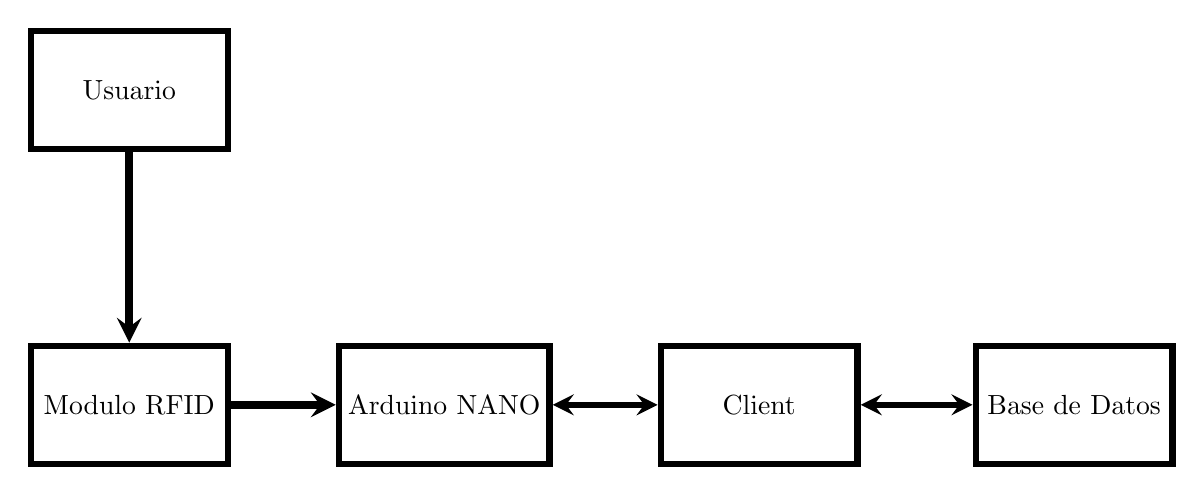
\begin{tikzpicture}[auto, node distance=2cm, >=stealth, line width=0.8mm]
    % Definición de bloques
    \node [draw, rectangle, minimum width=2.5cm, minimum height=1.5cm] (block1) {Modulo RFID};
    \node [draw, rectangle, minimum width=2.5cm, minimum height=1.5cm, right of=block1, node distance=4cm] (block2) {Arduino NANO};
    \node [draw, rectangle, minimum width=2.5cm, minimum height=1.5cm, right of=block2, node distance=4cm] (block3) {Client};
    \node [draw, rectangle, minimum width=2.5cm, minimum height=1.5cm, right of=block3, node distance=4cm] (block4) {Base de Datos};
    \node [draw, rectangle, minimum width=2.5cm, minimum height=1.5cm, above of=block1, node distance=4cm] (block5) {Usuario};



    % Flechas más grandes
    \draw[->, >=stealth, line width=1mm] (block1) -- (block2); % Grosor de la línea ajustado
    \draw[<->] (block2) -- (block3);
    \draw[<->] (block3) -- (block4);
    \draw[->, >=stealth, line width=1mm] (block5) -- (block1);
    
    
 
\end{tikzpicture}
\end{center}
\newpage
\section{Firmware}
\begin{enumerate}
    \item gpio.h:
    \lstinputlisting[language=Octave]{gpio.h}
    \item gpio.cpp:
    \lstinputlisting[language=Octave]{gpio.cpp}
    \newpage
    \item usart.h:
    \lstinputlisting[language=Octave]{usart.h}
    \item usart.cpp:
    \lstinputlisting[language=Octave]{usart.cpp}
\end{enumerate}


\newpage
\section{Core}
\begin{enumerate}
    \item Client.h
    \lstinputlisting[language=Octave]{Client.h}
    \item Client.cpp
    \lstinputlisting[language=Octave]{Client.cpp}
    \newpage
    \item Vehicle.h
    \lstinputlisting[language=Octave]{Vehicle.h}
    \newpage
    \item Vehicle.cpp
    \lstinputlisting[language=Octave]{Vehicle.cpp}
    \newpage
    \item Person.h
    \lstinputlisting[language=Octave]{Person.h}
    \item Person.cpp
    \lstinputlisting[language=Octave]{Person.cpp}
    \newpage
    \item Error.h
    \lstinputlisting[language=Octave]{Error.h}
    \item Error.cpp
    \lstinputlisting[language=Octave]{Error.cpp}
    \newpage
    \item Database.h
    \lstinputlisting[language=Octave]{Database.h}
    \item Database.cpp
    \lstinputlisting[language=Octave]{Database.cpp}
\end{enumerate}
\newpage
\section{Client}
\begin{enumerate}
    \item addcarddialog.h
    \lstinputlisting[language=Octave]{addcarddialog.h}
    \item addcarddialog.cpp
    \lstinputlisting[language=Octave]{addcarddialog.cpp}
    \newpage

    \item addvehicledialog.h
    \lstinputlisting[language=Octave]{addvehicledialog.h}
    \item addvehicledialog.cpp
    \lstinputlisting[language=Octave]{addvehicledialog.cpp}

    \item balancehandler.h
    \lstinputlisting[language=Octave]{balancehandler.h}
    \item balancehandler.cpp
    \lstinputlisting[language=Octave]{balancehandler.cpp}

    \item clientlistdialog.h
    \lstinputlisting[language=Octave]{clientlistdialog.h}
    \item clientlistdialog.cpp
    \lstinputlisting[language=Octave]{clientlistdialog.cpp}

    \item editclientdialog.h
    \lstinputlisting[language=Octave]{editclientdialog.h}
    \item editclientdialog.cpp
    \lstinputlisting[language=Octave]{editclientdialog.cpp}
    \item editvehicledialog.h
    \lstinputlisting[language=Octave]{editvehicledialog.h}
    \item editvehicledialog.cpp
    \lstinputlisting[language=Octave]{editvehicledialog.cpp}

    \item main.cpp
    \lstinputlisting[language=Octave]{main.cpp}
    \item mainwindow.h
    \lstinputlisting[language=Octave]{mainwindow.h}
    \item mainwindow.cpp
    \lstinputlisting[language=Octave]{mainwindow.cpp}



    \item serialhandler.h
    \lstinputlisting[language=Octave]{serialhandler.h}
    \item serialhandler.cpp
    \lstinputlisting[language=Octave]{serialhandler.cpp}
    \item vehiclelistdialog.h
    \lstinputlisting[language=Octave]{vehiclelistdialog.h}
    \item vehiclelistdialog.cpp
    \lstinputlisting[language=Octave]{vehiclelistdialog.cpp}
 
    
\end{enumerate}
\section{Server}


\end{document}
\end{document}
